\documentclass[10pt]{ctexart}

\usepackage[a4paper,margin=2.3cm]{geometry}
\usepackage{amsmath,amssymb,bm}
\usepackage{booktabs}
\usepackage[hidelinks]{hyperref}
\usepackage{graphicx}

\setlength{\parindent}{2em}
\setlength{\parskip}{0pt}

\begin{document}

\setcounter{section}{2}

\section{方法}

\paragraph{任务设定与目标。}
本文研究连续环境下的视觉语言导航（VLN-CE~\cite{vlnce}）：给定自然语言指令 $q$，机器人在每个时刻 $t$ 仅获得第一人称前视 RGB 观测 $I_t$，并在未知环境中执行移动，直至到达指令所描述的目标。记因果观测历史为 $\mathcal{O}_t=\{I_1,\ldots,I_t\}$，策略在每个决策时刻输出由 32 个 waypoint 组成的局部轨迹 $\mathcal{W}_t$，再经离散化执行。整个过程不提供 GT 位姿、深度或任何外部地图。

在此设定上，本文将\textbf{显式时空认知}定义为一个可监督的预测问题。对任一历史时刻 $\tau$，记其观测位姿在\emph{当前第一人称参考系}（以当前相机为原点、当前朝向为正前方）中的平面位置与朝向为 $\mathbf{x}_{t\leftarrow\tau}$。认知目标是从纯视觉历史逼近条件分布
\[
p\left(\mathbf{x}_{t\leftarrow\tau}\mid\mathcal{O}_t\right),
\qquad \tau\in\Gamma_t,
\]
其中 $\Gamma_t$ 为选定的至多 $K=8$ 个历史时刻。我们以四个规范方向 $\mathcal{V}=\{\mathrm{Front},\mathrm{Right},\mathrm{Back},\mathrm{Left}\}$ 拼成完整的第一人称全景参考系，并用各方向上的空间热力图与方向可见性作为该分布的离散参数化——即历史路点的 affordance map。$K$ 个历史路点的分布集合刻画了"哪些位置被访问过、它们如今在我的哪个方向、多远"，构成一种无需全局坐标系、以当前视点为锚的第一人称拓扑。由此，原本隐式的本体--环境时空记忆被转化为可学习、可监督、可观测的模型能力。

\paragraph{框架概览。}
围绕这一目标，本文方法由三部分组成：(1) 基于快慢系统的 VLA backbone，在统一框架内解耦长期高层意图与短期精细动作（3.1 节）；(2) 基于第一人称拓扑的显式时空认知机制，从历史 RGB 中估计相对位姿并预测历史路点的 affordance map（3.2 节）；(3) 时空认知与导航决策的关联学习，经共享计划表示将认知耦合进动作生成（3.3 节）。配套的结构化数据生成与分阶段优化在 3.4 节给出。整体框架如图~1 所示，记为 Past--Plan--Action（PPA），其信息流为
\[
\mathrm{History}
\longrightarrow
\mathrm{Plan}
\longrightarrow
\left\{
\mathrm{Future\ Heatmap},
\mathrm{Action\ Trajectory}
\right\},
\]
历史认知只沿时间因果方向汇入决策，历史与未来之间不存在反向通路。

\begin{figure}[h]
    \centering
    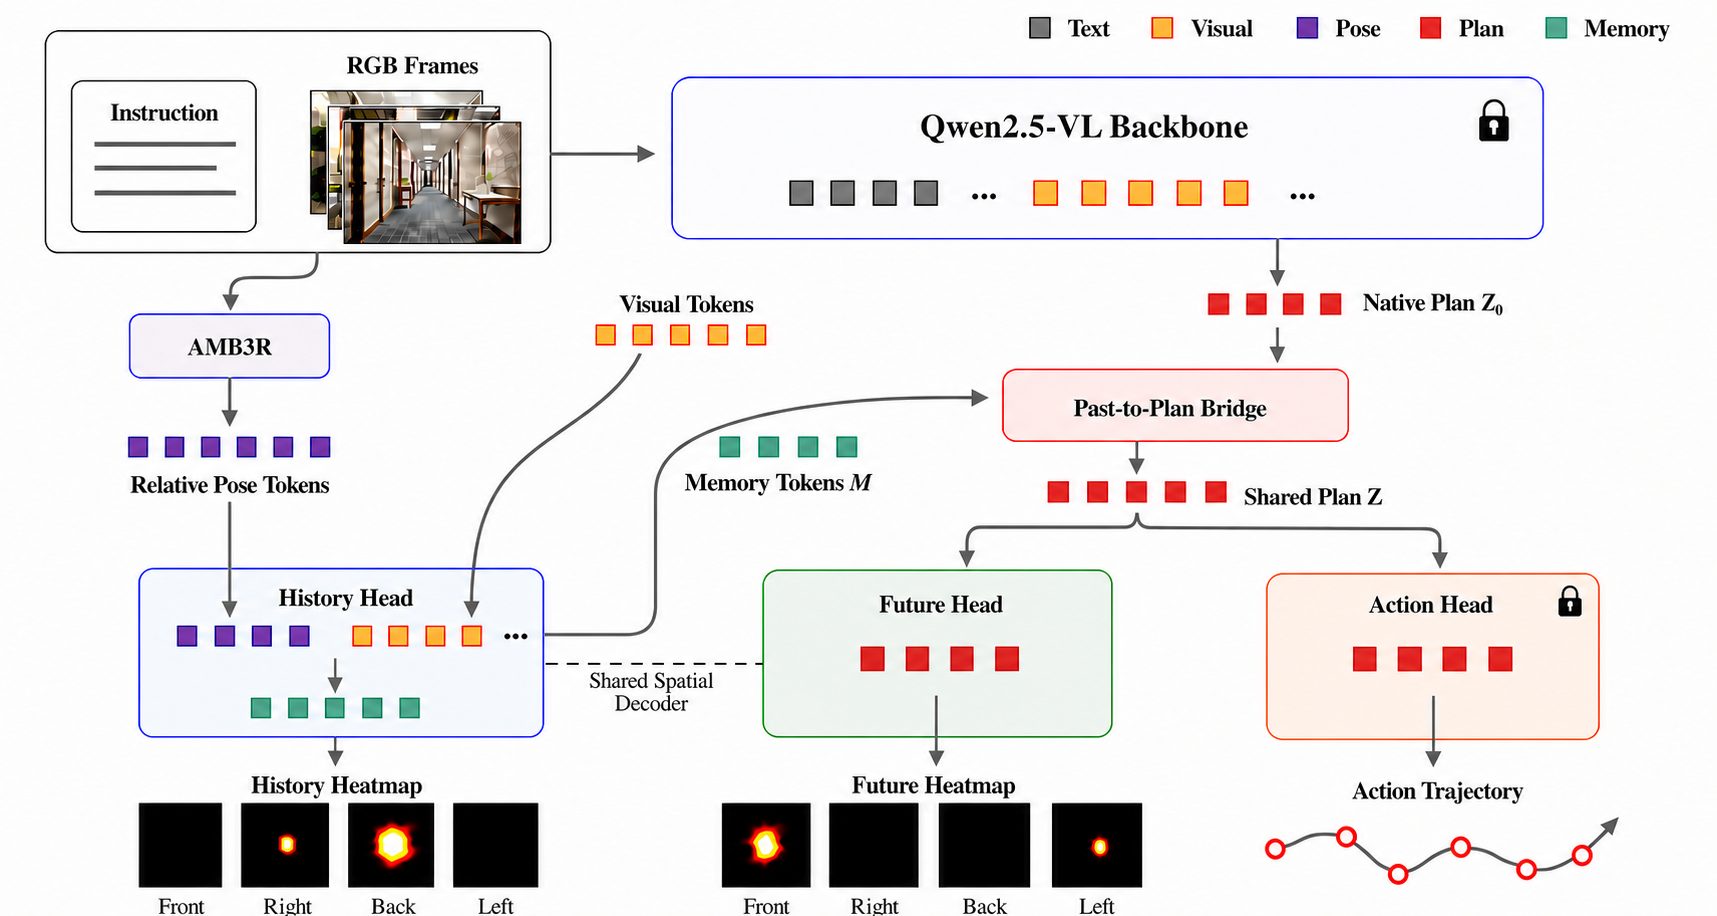
\includegraphics[width=1\linewidth]{figures/past_plan_action_main_overview_v6.png}
    \caption{Past--Plan--Action 整体框架。慢系统从指令与 RGB 历史生成原生 Plan $\mathbf{Z}^{0}$；相对位姿估计模块从同一 RGB 历史恢复历史观测的相对位姿；History Head 据此预测四方向历史 affordance map 并输出紧凑记忆 $\mathbf{M}$；Past-to-Plan Bridge 将 $\mathbf{M}$ 汇入 Plan 得到共享 Plan $\mathbf{Z}$；Future Head 与快系统的动作解码器并行读取 $\mathbf{Z}$，分别解码未来热力图与动作轨迹。History 与 Future 共享同一空间解码器。}
    \label{fig:overview}
\end{figure}

\subsection{基于快慢系统的 VLA Backbone}
\label{sec:backbone}

本文的 VLA backbone 遵循快慢系统设计：慢系统基于语言指令与观测历史推理长期的高层导航意图，快系统结合该意图与当前短期视觉状态生成精细动作，从而在统一框架内解耦不同时间尺度的决策与控制。慢系统执行完整的视觉语言推理，并将高层意图汇聚为四个 latent plan token；经条件投影 $\phi_{\mathrm{cond}}$ 后得到
\[
\mathbf{Z}^{0}_t
=
\phi_{\mathrm{cond}}
\bigl(
\mathrm{Slow}(q,\mathcal{O}_t)
\bigr)
\in
\mathbb{R}^{4\times768},
\]
记为\textbf{原生 Plan}。它是慢系统对"接下来应当去哪里"的意图表示；停止判定同样由慢系统给出。快系统是一个 flow-matching 轨迹解码器，以 Plan 为条件、结合当前视觉状态 $\mathbf{J}_t$ 生成 32 个 waypoint 的局部轨迹，推理时沿用多样本生成、轨迹聚合与离散动作后处理。

我们将该 backbone 实例化于预训练的 InternNav~\cite{internnav} 双系统模型：慢系统对应其 System-2（Qwen2.5-VL~\cite{qwen25vl} 规划器），快系统对应其 System-1（NextDiT 轨迹扩散模块）。骨干在本文全部训练阶段保持冻结——学习容量由此集中于时空认知及其与决策的耦合，性能变化也可严格归因于认知的引入。

该 backbone 有一个对本文至关重要的结构性质：\textbf{Plan 是慢系统与快系统之间唯一的意图通道}。显式时空认知因此不必侵入骨干内部，只需修正这四个 Plan token 即可影响后续行为。引入认知模块后的整体前向为
\begin{equation}
\begin{aligned}
\mathbf{Z}^{0}_t
&=
\phi_{\mathrm{cond}}
\bigl(
\mathrm{Slow}(q,\mathcal{O}_t)
\bigr),\\
\bigl(
\widehat{\mathcal{H}}^{\mathrm{hist}}_t,
\widehat{\bm{\ell}}^{\mathrm{hist}}_t,
\mathbf{M}_t
\bigr)
&=
\mathrm{HistoryHead}
\bigl(
\mathcal{O}_t,\widehat{\mathbf{P}}_t
\bigr),\\
\mathbf{Z}_t
&=
\mathbf{Z}^{0}_t+
\mathrm{Bridge}
\bigl(
\mathbf{Z}^{0}_t,\mathbf{M}_t
\bigr),\\
\bigl(
\widehat{\mathcal{H}}^{\mathrm{fut}}_t,
\widehat{\bm{\ell}}^{\mathrm{fut}}_t
\bigr)
&=
\mathrm{FutureHead}
\bigl(
\mathbf{Z}_t,\mathbf{F}_t
\bigr),\\
\widehat{\mathcal{W}}_t
&=
\mathrm{ActionHead}
\bigl(
\mathbf{Z}_t,\mathbf{J}_t
\bigr),
\end{aligned}
\label{eq:overview}
\end{equation}
其中 $\widehat{\mathbf{P}}_t$ 为从 RGB 历史估计的相对位姿（3.2 节），$\widehat{\mathcal{H}}$、$\widehat{\bm{\ell}}$ 分别为历史/未来热力图及其方向可见性，$\mathbf{M}_t$ 为紧凑历史记忆，$\mathbf{F}_t$ 为空间解码复用的当前视觉特征。历史信息只通过四个共享 Plan token 影响未来空间预测与动作生成。

\subsection{基于第一人称拓扑的显式时空认知}
\label{sec:cognition}

\paragraph{因果相对位姿估计。}
显式时空认知的前提是回答"历史观测相对当前视角在哪里"。本文将其化为纯 RGB 的前馈推断：采用 AMB3R~\cite{amb3r} 作为因果几何模块，顺序处理已观测的前视图像前缀并输出各帧位姿，借助中间帧维持远距离历史与当前帧之间的几何关联。History Head 只从中选择 $\Gamma_t$ 中至多 $K$ 个时刻作为输出槽，位姿估计的时间分辨率与输出槽数相互独立。设 $\widehat{\mathbf{T}}_i$ 为估计的 camera-to-world 位姿，历史时刻 $\tau_k$ 相对当前的变换及其平面表示为
\begin{equation}
\widehat{\mathbf{T}}_{t\leftarrow\tau_k}
=
\widehat{\mathbf{T}}_t^{-1}
\widehat{\mathbf{T}}_{\tau_k},
\qquad
\widehat{\mathbf{p}}_{t\leftarrow\tau_k}
=
\left[
\Delta\widehat f_k,\,
\Delta\widehat l_k,\,
\cos\Delta\widehat\psi_k,\,
\sin\Delta\widehat\psi_k
\right],
\label{eq:relative_pose}
\end{equation}
其中 $\Delta\widehat f_k$、$\Delta\widehat l_k$ 为当前机器人坐标系中的前向与左向位移，$\Delta\widehat\psi_k$ 为相对航向角。相对表示消除了世界坐标原点的影响，正余弦形式避免了航向角在 $\pm\pi$ 处的不连续。推理阶段该模块只读取 RGB；GT 位姿、深度与内参仅用于监督标签构造与离线评测（3.4 节），从不作为模型输入。

\paragraph{历史编码与四方向规范槽。}
History Head 复用骨干的视觉编码器（不重复执行语言推理）：当前图像保留多层二维空间特征以支持像素级定位，每张历史图像压缩为一个紧凑视觉 token 以描述该次观测的外观与身份。空间支路在四个规范方向上组织：Front 槽直接采用当前前视图的真实空间特征；Right、Back、Left 槽由可学习的规范空间查询、方向编码与前视全局上下文构成——它们是带方向语义的规范空间槽，而非合成的侧后视图。

\paragraph{轨迹引导的时空关联。}
History Head 的整体机制如图~2 所示。对第 $k$ 个历史槽，相对位姿 $\widehat{\mathbf{p}}_{t\leftarrow\tau_k}$ 经 Fourier 编码与线性投影形成 trajectory token，与历史视觉 token、四方向空间 token 一同输入两层 trajectory-guided Transformer：历史 token 回答"这是哪次观测"，trajectory token 回答"它相对当前在哪里"，空间 token 承载规范视角中的像素布局。三者在同一注意力空间中联合更新，迫使模型建立历史观测之间的时空关联。更新后的历史 token $\mathbf{h}'_{t,k}\in\mathbb{R}^{256}$ 预测该路点的四方向 visibility，并被保留为 compact memory $\mathbf{m}_{t,k}=\mathbf{h}'_{t,k}$；更新后的空间 token 先解码 $8\times8$ 的 coarse heatmap，再由 Fine Decoder 结合当前图像多尺度特征细化为最终热力图：
\[
\widehat{\mathcal{H}}^{\mathrm{hist}}_t
\in
\mathbb{R}^{K\times4\times64\times64},
\qquad
\mathbf{M}_t=[\mathbf{m}_{t,1},\ldots,\mathbf{m}_{t,K}]
\in
\mathbb{R}^{K\times256}.
\]
训练与后续共享解码均保留原始 logits，以保存峰值宽度、多峰结构与方向不确定性；可视化与评测时再将方向概率与方向内空间概率组合为全景热力图。$\mathbf{M}_t$ 是历史表征与 Plan 之间的唯一通信接口；无效历史槽在损失与注意力中一并屏蔽，无任何有效槽时系统精确退化为原生骨干（附录~B）。

\begin{figure}[h]
    \centering
    \fbox{\begin{minipage}{0.93\linewidth}\small
    \textbf{【图待制作——内容规格】}History Head 机制图：
    (i) 左侧输入列：当前前视 RGB $\rightarrow$ 空间特征（Front 槽）与可学习 Right/Back/Left 规范槽；$K$ 张历史 RGB $\rightarrow$ 紧凑历史 token；相对位姿 $\rightarrow$ Fourier $\rightarrow$ trajectory token。
    (ii) 中部：每个历史槽的 $[\,$历史 token、trajectory token、$4\times8\times8$ 空间 token$\,]$ 进入两层 Transformer 联合更新（画出 token 序列与自注意力）。
    (iii) 右侧三条输出支路：历史 token $\rightarrow$ visibility 与 compact memory $\mathbf{m}_{t,k}$（标注"$\rightarrow$ Bridge"）；空间 token $\rightarrow$ coarse $8\times8$ $\rightarrow$ Fine Decoder（融合当前多尺度特征）$\rightarrow$ $4\times64\times64$ affordance map。
    配色沿用图~1 的 token 色系（Visual/Pose/Memory）。
    \end{minipage}}
    \caption{History Head：从历史观测与相对位姿到第一人称 affordance map 与紧凑记忆。}
    \label{fig:historyhead}
\end{figure}

\subsection{时空认知与导航决策的关联学习}
\label{sec:association}

显式时空认知若只是独立的辅助任务，则无法保证真正服务于导航。本节机制让认知结果直接参与行为生成，同时遵循一条设计原则：\textbf{认知增强不得破坏骨干的原生能力}。关联仅沿时间因果方向发生——历史记忆经 Bridge 汇入 Plan，未来预测与动作生成从同一共享 Plan 读取，反向通路不存在。

\paragraph{Past-to-Plan Bridge。}
Bridge 用一次多头交叉注意力将 compact memory 传递给原生 Plan：
\begin{equation}
\begin{aligned}
\Delta\mathbf{Z}_t
&=
\mathbf{W}_{o}\,
\operatorname{MHA}
\left(
\operatorname{LN}(\mathbf{Z}^{0}_t),
\operatorname{LN}(\mathbf{M}_t),
\operatorname{LN}(\mathbf{M}_t)
\right),\\
\mathbf{Z}_t
&=
\mathbf{Z}^{0}_t+\Delta\mathbf{Z}_t,
\end{aligned}
\label{eq:bridge}
\end{equation}
输出投影 $\mathbf{W}_{o}$ 零初始化，因此训练起点处 $\mathbf{Z}_t=\mathbf{Z}^{0}_t$，新分支不会立即扰动原生动作条件，而 $\mathbf{W}_{o}$ 在首次反传即获得有效梯度。在此之上，Bridge 对每个 Plan token 的修正量施加硬信任域：
\begin{equation}
\Delta\mathbf{z}
\leftarrow
\Delta\mathbf{z}\cdot
\min\!\left(
1,\;
\frac{\rho\,\|\mathbf{z}^{0}\|}{\|\Delta\mathbf{z}\|}
\right),
\qquad
\rho=0.05,
\label{eq:trust_region}
\end{equation}
即修正范数不超过对应原生 token 范数的 $5\%$，训练与部署一致生效。该约束从结构上保证共享 Plan 始终处于原生意图的邻域内。Bridge 只作用于四个 Plan token，不在动作解码器内部插入逐层条件支路。

\paragraph{Future Head：历史与未来的统一空间语义。}
历史路点以 affordance map 表达后，慢系统的未来意图可以在同一空间语义下解释。Future Head 直接读取四个共享 Plan token——其本身不含注意力模块，仅由线性投影、类型与时段嵌入、可学习空间查询及共享解码头构成，因此三个输出头之间的全部关联都发生在共享 Plan 上。expert 局部轨迹重采样为 32 个 waypoint 并按进度分为四段（$1$--$8$、$9$--$16$、$17$--$24$、$25$--$32$），四个 Plan token 分别解码对应时间段在四个规范方向中的空间 tube：
\[
\widehat{\mathcal{H}}^{\mathrm{fut}}_t
\in
\mathbb{R}^{4\times4\times64\times64},
\]
每个 tube 描述一段未来轨迹的空间支持区域而非单个目标点。History 与 Future 共享四方向 visibility 头、coarse 头与空间细化主干，各自保留输入适配与输出投影（完整清单见附录~B）。由此，"我从哪里来"与"我要到哪里去"在同一四方向规范坐标系中共享几何词汇，历史与未来的时空关系得以在共享 Plan 上直接关联。

\paragraph{与动作生成的耦合。}
动作解码器同样以共享 Plan $\mathbf{Z}_t$ 为条件生成局部轨迹。三个输出头之间不存在显式铰链：Future 的预测不输入动作解码器，动作轨迹也不回写 History；耦合来自对同一共享 Plan 的并行读取，以及训练中施加其上的历史、未来与动作监督（3.4 节）。动作解码器参数虽不更新，其输出对 Plan 的梯度仍回传至 Bridge 与 History Head，动作监督由此参与塑造时空记忆本身。热力图作为监督与可解释输出，不以解码后的像素形式回流进策略。三个头的关系可概括为：History 提供过去的空间记忆，Bridge 将其汇入当前 Plan，Future 解释该 Plan 的未来展开，动作解码器将同一 Plan 变为可执行轨迹。

\subsection{结构化数据生成与分阶段优化}
\label{sec:training}

显式时空认知没有现成的监督来源，本文以结构化的数据自动生成流程构造之，并以分阶段优化使时空理解、高层意图与低层控制逐步协同。

\paragraph{结构化数据自动生成。}
训练数据基于 VLN-CE 的 R2R expert 轨迹自动构建：在 Habitat 中回放 expert episode，采集全景观测（四方向 RGB、深度）与相机位姿；模型输入只使用前视 RGB，全景信息仅服务于标签构造与评测。每条轨迹按时间步展开为因果滑动窗口样本，每个样本以当前时刻为参考、从历史前缀中采样至多 $K$ 个历史槽。全部监督标签自动生成（图~3）：

\begin{itemize}
    \item \textbf{历史标签}：将各历史相机中心经 GT 位姿变换到当前坐标系，投影至四个规范方向，结合深度做遮挡与可见性判定，以自适应空间核栅格化为热力图标签；
    \item \textbf{未来标签}：由 32 个重采样 waypoint 的三维相对几何生成（不使用未来帧与 GT 深度），平坦路段取与当前相机同高的相对高度、楼梯等垂直运动保留 expert 相对高度，再按时间段投影并栅格化为 tube；
    \item \textbf{因果位姿缓存}：对每条轨迹按与在线推理一致的因果前缀流程离线运行位姿估计并缓存，训练输入 $100\%$ 使用估计位姿而非 GT，使 History Head 在训练期即适配推理时的位姿误差分布。
\end{itemize}

数据划分采用确定性的场景级散列，训练与验证场景不相交。投影、可见性判定、核函数与重采样细节见附录~A。

\begin{figure}[h]
    \centering
    \fbox{\begin{minipage}{0.93\linewidth}\small
    \textbf{【图待制作——内容规格】}结构化标签生成示意图，左右两栏：
    (i) 左栏"历史标签"：俯视小地图画出 expert 轨迹与历史相机位置、当前位姿及其四方向视锥；向下箭头到四张 $64\times64$ 标签热力图（可见方向为高斯峰、被遮挡方向标记不可见），标注"GT 位姿/深度仅在此处使用"。
    (ii) 右栏"未来标签"：同一俯视图上画 32 个重采样 waypoint 按四个时间段着色；向下箭头到 $4\times4$ 网格的 tube 标签（每行一个时间段、每列一个方向）。
    (iii) 底部横条"因果位姿缓存"：时间轴上顺序 ingest 的 RGB 前缀 $\rightarrow$ 估计位姿行，标注"与在线推理同分布"。
    \end{minipage}}
    \caption{结构化数据自动生成：历史 affordance map 标签、未来轨迹 tube 标签与因果位姿缓存均从 expert 轨迹自动构造，无需人工标注。}
    \label{fig:labels}
\end{figure}

\paragraph{训练目标。}
History 的监督目标 $\mathcal{L}_{\mathrm{hist}}$ 包含四方向 visibility、热力图空间定位（含 soft-argmax 坐标项）、不可见方向抑制与方向不均衡校正；验证使用可见性、PCK 与像素定位误差。Future tube 可跨越多个方向，故 $\mathcal{L}_{\mathrm{fut}}$ 不含单点坐标项与互斥视角分类，由 visibility、tube 空间分布、不可见抑制与方向均衡项组成；Soft-IoU、top-$k$ support recall 与 visibility F1 仅作验证指标。各项权重见附录~C。

\paragraph{分阶段优化。}
训练策略围绕一对内在张力展开：时空认知必须\emph{参与}决策（需要动作梯度流入认知分支），又必须\emph{不破坏}骨干先验（expert 监督中存在大量不可约的多模态残差，若不加约束地推动 Plan，模型会为微小的 teacher-forced 增益漂移出原生意图邻域，损害闭环行为）。本文以三个阶段化解该张力，从空间对齐、到受保护的耦合、再到信任域内收敛。历史空间分支在此前已完成预训练与位姿域适配（从 GT 位姿切换到估计位姿分布），作为初始化。

\textbf{Stage 1（历史--未来空间对齐）}保持 Bridge 为零映射（$\mathbf{Z}_t=\mathbf{Z}^{0}_t$），训练历史分支的轨迹引导 Transformer 与输入投影、Future Head 及共享解码头：
\begin{equation}
\mathcal{L}_{\mathrm{stage1}}
=
\lambda_h\mathcal{L}_{\mathrm{hist}}
+
\lambda_f\mathcal{L}_{\mathrm{fut}}.
\label{eq:stage1}
\end{equation}
保留 History loss 使未来 tube 解码的学习不侵蚀已有的历史定位能力，并让历史与未来预测在同一规范坐标系中完成参数对齐。

\textbf{Stage 2（认知--决策联合训练）}启用零初始化的 Bridge，联合更新认知分支与 Bridge。除动作目标 $\mathcal{L}_{\mathrm{act}}$（flow matching）外，加入 native preservation loss：对同一组 noisy trajectory 与扩散时间步，分别以共享 Plan 和原生 Plan 计算动作解码器的速度预测并约束一致，
\begin{equation}
\mathcal{L}_{\mathrm{pres}}
=
\left\|
\mathbf{V}_{\mathrm{act}}
\left(
\mathbf{X}_s,s,\mathbf{Z}_t,\mathbf{J}_t
\right)
-
\operatorname{sg}
\left[
\mathbf{V}_{\mathrm{act}}
\left(
\mathbf{X}_s,s,\mathbf{Z}^{0}_t,\mathbf{J}_t
\right)
\right]
\right\|_2^2,
\label{eq:preservation}
\end{equation}
两条支路共享同一组噪声与时间步（$\operatorname{sg}$ 为停止梯度）。总目标为
\begin{equation}
\mathcal{L}_{\mathrm{stage2}}
=
\lambda_a\mathcal{L}_{\mathrm{act}}
+
\lambda_h\mathcal{L}_{\mathrm{hist}}
+
\lambda_f\mathcal{L}_{\mathrm{fut}}
+
\lambda_p\mathcal{L}_{\mathrm{pres}}
+
\lambda_{\Delta}
\left\|
\mathbf{Z}_t-\mathbf{Z}^{0}_t
\right\|_2^2.
\label{eq:stage2}
\end{equation}

\textbf{Stage 3（信任域内的桥接收敛）}处理上述张力中最关键的一环：动作残差的主体是不可约的多模态噪声，均匀的动作监督会将其转化为对 Plan 的持续漂移压力。为此，Stage 3 冻结全部热力图分支，将 Bridge 重置为零态后在信任域内单独重训，并作三项重构：(i) 启用式~\eqref{eq:trust_region} 的硬信任域，将残差惩罚替换为逐 token 的尺度无关形式 $\|\Delta\mathbf{z}\|^2/\|\mathbf{z}^{0}\|^2$，并以 preservation 为主导权重，使"静默 Bridge"成为无增益方向上的默认最优解；(ii) 以 advantage 加权动作损失，
\begin{equation}
w
=
\min\!\left(
\frac{
\bigl\|
\mathbf{V}_{\mathrm{act}}(\mathbf{X}_s,s,\mathbf{Z}^{0}_t,\mathbf{J}_t)-\mathbf{V}^{\ast}
\bigr\|_2^2
}{
m_{\mathrm{ref}}
},\;
c
\right),
\label{eq:advantage}
\end{equation}
动作监督仅在原生快系统确实出错的样本上（原生速度误差超出参考水平 $m_{\mathrm{ref}}$）向 Bridge 施压；(iii) checkpoint 依据真实采样 rollout 的端点误差选择——在共享噪声与一致的部署后处理下对比桥接与原生轨迹，而非 teacher-forced 误差。小权重的未来空间监督经共享 Plan 继续约束桥接方向，保持修正的空间可解释性。无约束桥接对闭环性能的破坏在实验部分通过消融量化。

\paragraph{推理。}
推理时模型只读取指令与截至当前的 RGB：估计相对位姿、生成历史 affordance map 与 compact memory、在信任域内形成共享 Plan，随后并行解码未来热力图与动作轨迹。热力图用于可视化与诊断，不回流进策略。

\begin{thebibliography}{9}

\bibitem{internnav}
M. Wei et al.
\newblock Ground Slow, Move Fast: A Dual-System Foundation Model for
Generalizable Vision-and-Language Navigation.
\newblock 2025.

\bibitem{amb3r}
H. Wang and L. Agapito.
\newblock AMB3R: Accurate Feed-forward Metric-scale 3D Reconstruction
with Backend.
\newblock 2025.

\bibitem{qwen25vl}
S. Bai et al.
\newblock Qwen2.5-VL Technical Report.
\newblock 2025.

\bibitem{vlnce}
J. Krantz, E. Wijmans, A. Majumdar, D. Batra, and S. Lee.
\newblock Beyond the Nav-Graph: Vision-and-Language Navigation in
Continuous Environments.
\newblock In ECCV, 2020.

\end{thebibliography}

\section*{附录 A：标签构造细节}

\paragraph{四方向规范参考系。}
以当前相机为原点、当前朝向为正前方，四个规范方向对应偏航角 $0^{\circ}$（Front）、$-90^{\circ}$（Right）、$180^{\circ}$（Back）、$+90^{\circ}$（Left），各自以针孔模型投影到 $64\times64$ 网格。

\paragraph{历史标签。}
对历史时刻 $\tau_k$，将其相机中心经 GT 位姿变换到当前坐标系，分别投影至四个规范方向；落在视锥内的方向进行深度遮挡测试（沿投影射线比较该方向深度图），通过者记为可见。可见方向以该投影点为中心、按投影几何自适应确定 $\sigma$ 的高斯核栅格化为空间标签；不可见方向仅提供负类 visibility 标签。标签在数据加载阶段按样本即时构造，GT 位姿、深度与内参不进入模型输入。

\paragraph{未来标签。}
未来监督由 expert 局部轨迹的 32 个重采样 waypoint 生成。平坦路段的 waypoint 高度取为与当前相机同高（相对高度为零）；对楼梯、电梯等存在垂直运动的片段，按动作对齐插值保留 expert 轨迹中的相对高度变化。每个时间段（8 个 waypoint）投影到四个规范方向后，以每 waypoint 一个高斯（三维支撑尺度 $1.5\,\mathrm{m}$，像素域 $\sigma\in[4,8]$）叠加栅格化为 tube 标签，并配套各时间段$\times$方向的 visibility 标签与时间段有效掩码。全程不使用未来帧图像与 GT 深度。

\paragraph{因果位姿缓存。}
离线缓存严格复现在线推理的因果流程：每条轨迹从头顺序 ingest 前视 RGB（前 20 帧初始化，其后增量建图），在各地图更新端点处快照当帧的全前缀估计位姿；快照先于任何后续帧的 ingest，未来信息不可能泄漏进早期训练行。缓存不做逐 episode 的尺度标定。训练数据加载器只接受该缓存（缺失即报错），不存在回退到 GT 位姿的路径。

\section*{附录 B：模块细节与冻结策略}

\paragraph{模块--实现对照。}
慢系统为 InternNav System-2（Qwen2.5-VL 视觉语言规划器）；快系统为 InternNav System-1（12 层 NextDiT flow-matching 解码器，隐藏维 384，动作维 3，32 步）；条件投影 $\phi_{\mathrm{cond}}$ 为骨干原生的两层 MLP（$3584\!\to\!768$）。History Head 的视觉支路复用 Qwen2.5-VL 的视觉编码器：当前帧 hook 第 $\{7,15,23,31\}$ 层 ViT 特征（$1280$ 维、$16\times16$ 栅格）经 DPT 式融合；每张历史帧取 visual-merger 输出 token 的空间均值（$3584$ 维）。相对位姿四分量除以 $10$ 后作 16 频带正余弦编码（含原值共 $132$ 维），线性投影到融合维 $256$。每个历史槽的 token 序列为 $[\,$历史 token、trajectory token、$4\times8\times8$ 空间 token$\,]$ 共 258 个，经 2 层、4 头、FFN 1024 的 Transformer 编码器联合更新。

\paragraph{Bridge。}
多头交叉注意力（8 头，query 维 768，key/value 维 256），query/key/value 投影保持默认初始化，输出投影权重与偏置零初始化；query 侧与 key/value 侧各有独立 LayerNorm。该分支以 FP32 计算并禁用混合精度。无效历史槽经 key padding mask 屏蔽；当样本不存在有效历史槽时跳过注意力计算，输出与原生 Plan 逐比特一致。信任域截断（式~\ref{eq:trust_region}）在缩放系数封顶为 1 的形式下实现，零修正保持精确为零。

\paragraph{History/Future 参数共享清单。}
共享模块：四方向 visibility MLP、coarse heatmap MLP、Fine Decoder 空间细化主干（Future 经函数式调用替换最后一层输出投影）。History 专属：trajectory-guided Transformer、历史/空间 token 输入投影与位置嵌入。Future 专属（共 11 个张量）：Plan 投影、future 类型嵌入、4 个时间段嵌入、可学习空间查询（$4\times8\times8\times256$）、summary/spatial 两个 LayerNorm、future 输出投影。

\paragraph{精确行为边界。}
(i) Right/Back/Left 规范槽不读取任何侧后 RGB，方向编码为固定角基经可学习两层 MLP；(ii) coarse heatmap 由空间 token 解码，compact memory 不直接预测热力图，二者经联合注意力共享历史表征；(iii) 空间监督只施加在 $64\times64$ 的 fine logits 上，coarse 图作为 Fine Decoder 的中间输入间接受约束；(iv) preservation 的两条支路必须共享同一组噪声与时间步，否则目标退化为对随机性的拟合；(v) 历史与未来热力图的解码结果不以任何显式控制信号回流进动作解码器。

\paragraph{各阶段冻结策略。}
骨干（慢系统、视觉编码器、条件投影、动作解码器）在所有阶段冻结。历史分支的多尺度特征融合与四方向规范槽构造在预训练与位姿域适配阶段训练，进入 Stage 1--3 后冻结继承。各阶段可训练集合：Stage 1 为历史分支的 Transformer 与输入投影、Future Head、共享解码头；Stage 2 在此之上加 Bridge；Stage 3 仅 Bridge（自零态重训）。

\section*{附录 C：训练超参数}

\begin{table}[h]
\centering
\small
\begin{tabular}{lccc}
\toprule
 & Stage 1 & Stage 2 & Stage 3 \\
\midrule
$\lambda_a$（action） & --- & $1.0$ & $1.0$（advantage 加权） \\
$\lambda_h$（history） & $0.3$ & $0.3$ & $\approx0$ \\
$\lambda_f$（future） & $0.3$ & $0.3$ & $0.1$ \\
$\lambda_p$（preservation） & --- & $0.5$ & $2.0$ \\
$\lambda_{\Delta}$（plan 残差） & --- & $0.01$（绝对） & $10$（相对 $\|\Delta\mathbf{z}\|^2/\|\mathbf{z}^0\|^2$） \\
信任域 $\rho$ & --- & --- & $0.05$ \\
advantage（$m_{\mathrm{ref}}$ / $c$） & --- & --- & $0.125$ / $4$ \\
可训练模块 & 认知分支+共享头 & +Bridge & 仅 Bridge（重置为零） \\
epoch & 4 & 4 & 3 \\
选点指标 & 历史/未来验证指标 & 验证综合指标 & 采样 rollout 端点误差 \\
\bottomrule
\end{tabular}
\caption{分阶段损失权重与训练设置。}
\label{tab:hparams}
\end{table}

学习率（AdamW，weight decay $10^{-2}$）：Stage 1 中 Future Head $10^{-4}$、历史分支 $2\times10^{-5}$、Fine Decoder $5\times10^{-6}$；Stage 2 相应降为 $5\times10^{-5}$、$10^{-5}$、$5\times10^{-6}$，Bridge $2\times10^{-5}$；Stage 3 中 Bridge $10^{-5}$。全局 batch 为 8（8 卡$\times$每卡 1$\times$无累积），训练维护 EMA 权重。历史监督内部权重：visibility $1.0$（正类权重 $7$）、空间 CE $1.0$、soft-argmax 坐标 $0.2$、不可见抑制 $0.25$、视角宏平衡 $0.5$、方向宏平衡 $0.5$、全景视角分类 $1.0$；未来监督权重：visibility $1.0$（正类权重 $1$）、tube 空间分布 $1.0$、不可见抑制 $0.25$、视角宏平衡 $0.5$，坐标项与方向宏平衡项置零。历史槽数 $K\in[5,8]$（每样本至少 5 个有效历史帧）。

\end{document}
